\section{Overall Discussion of Experiments}
\label{sec:ExperimentsDisucssion}

% ##############################################################################

In light of what we have presented so far, we have to acknowledge that the utilization of \gls{reid} in object tracking is not as useful as we had initially hypothesized. Nonetheless, we believe that similarity learning, on which the Siamese tracking paradigm itself is based, is of paramount importance to tracking. The recent advancements in Siamese tracking that our survey~\cite{ondrasovic2021siamese} covers directly support this claim. Despite the fact that \gls{reid} relies on similarity learning, the underlying architecture of the tracker needs to be taken into account.

The first experiment with external \gls{reid} model failed because of conflicting embedding vectors.

Based on the knowledge we have acquired via studying Siamese tracking, our recommendation is the following.

Our three documented Siamese-related experiments utilized the \uadetrac{} dataset only. To the best of our knowledge, this dataset is the closest one to traffic analysis domain with such a high quality of annotations and quantity of frames while using a static camera. Although our implementations turned out to be useful for general object tracking, we still continued using this dataset because of its size and the availability of annotations both for training and testing, with the latter being the primary reason.

We contemplated using the \motseventeen{} benchmark dataset (\sectiontext{}~\ref{ssec:DatasetMOT17},~p.~\pageref{ssec:DatasetMOT17}) on which the original \gls{siammot} model was trained and tested so as to directly compare our implementation with the published scores. However, the experiments we conducted would have been impossible to accomplish to such an extent had we relied exclusively on the \motseventeen{} evaluation. This dataset provides seven video sequences aimed at tracking people. Unlike the \uadetrac{} benchmark, the annotations for the test part of the \motseventeen{} are inaccessible. Thus, a validation set has to be produced from the training data. Even though this is a standard practice in machine learning, we could not successfully adopt it because the given seven sequences are significantly different from each other. We tried a cross-validation approach, \ietext{}, training on six sequences while the remaining one would be used for validation (and repeating for all combinations), but to no avail. A $5$/$2$ split did not work either. The \gls{mota} performance score on the validation set oscilated around $30$\%, which reduced our confidence in the obtained results. Furthermore, we have not seen using the training set of the \motseventeen{} dataset like this. The standard protocol is to train the model on the full training set, and then submit the inference output on the test data to the server for evaluation. But, as demonstrated in \sectiontext{}~\ref{ssec:DSAExperimentalEvaluation}, we would need dozens of evaluation runs. Such attempts would, according to the official rules, result in being banned from the server. Therefore, we had to rely on a dataset that provided annotations for all sequences. Likewise, we had the very same reasons for not using the \kitti{} dataset (\sectiontext{}~\ref{ssec:DatasetKITTIObjectTracking},~p.~\pageref{ssec:DatasetKITTIObjectTracking}).

% ------------------------------------------------------------------------------
\begin{figure}[t]
    \centerline{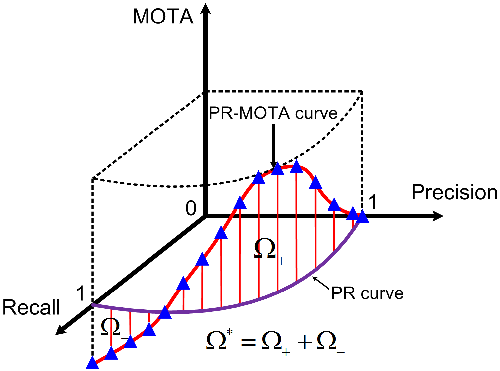
\includegraphics[width=0.5\linewidth]{figures/siamese_tracking/pr_mota_curve.pdf}}
    \caption[Visualization of \gls{mota} along a precision-recall curve]{Visualization of the \gls{mota} metric extended to third dimension along a precision-recall curve developed as part of the \uadetrac{} benchmark. \externalsrc{\cite{wen2020uadetrac}}}
    \label{fig:PRMOTAVisualization}
\end{figure}
% ------------------------------------------------------------------------------

The \uadetrac{} provides a leaderboard on its own. However, the authors of this dataset proposed new evaluation metrics that are coincidentally inappropriate for our framework, rendering our endeavor to enter the ranking unattainable. They extended the \gls{mota} and \gls{motp} metrics into third dimension by evaluating them along a precision-recall curve and then computing an area under the obtained curve (\figtext{}~\ref{fig:PRMOTAVisualization}). We do agree with their justification for introducing another metric as well as the method itself. Nevertheless, the precision-recall curve is used to evaluate object detection by altering the threshold value indicating whether a prediction is correct or not. In the case of \gls{siammot}, this is not possible to achieve easily, if at all. Even the official \uadetrac{} leaderboard contains tracking approaches that adopt the ``detection + linking'' paradigm. In such a setup, the detector itself is an isolated module the output of which is processed by a ``linker'', \egtext{}, some graph-based optimization algorithm. The generation of precision-recall curve is easily produced by altering the threshold over the detector predictions. All it then takes is to run multiple evaluations of the linking phase over several detector predictions. On the other hand, the \gls{siammot} utilizes three threshold values, namely the minimum value for the track to start, to stay active or to become resumed from dormant state. Even if we had found a way to emulate the evaluation protocol, we would have done so in an intricate way the credibility of which could be questioned.

Considering this, the use of \gls{clear} metrics (\sectiontext{}~\ref{sec:EvaluatingMOT},~p.~\pageref{sec:EvaluatingMOT}) on top of the \uadetrac{} dataset provided the best combination of traffic-related data with established and widely adopted metrics. After all, the objective was to compare our extensions with the original model in relative terms, and for that our approach served sufficiently.
